\documentclass[aspectratio=169,11pt]{beamer}

% ================================================================
% "TABIIY TILNI QAYTA ISHLASH" KURSI
% MA'RUZA 15 --- Sun'iy intellekt agentlarini yaratish (ReAct, LangChain)
%              (d15_agentlar.tex)
% Arxetiplar: [A][B][C][D][E] + 4 tsikl [F][G][H][I][J][K][L] +
%             [M][N][O][P][Q][R] + ilova [S]
% Rendered slayd soni: ~47 (4-haftaning agent ma'ruzasi; L1-L14 chuqurligi)
% Qulflangan [I1]: ReAct tool tanlash --- correct_tool=sentiment_classify, conf=0.82>0.7
%   --- P15 (Day 16) birinchi assert manbayi (course_map hand_example).
% MUHIM ARK: L14 RAG bitta vosita -> L15 agent ko'p vositani rejalashtirib chaqiradi.
% ================================================================

% ================================================================
% RANGLAR  (asl fayldan o'zgarishsiz)
% ================================================================
\definecolor{cnublue}{rgb}{0.07,0.14,0.62}
\definecolor{cnubluelight}{rgb}{0.18,0.30,0.72}
\definecolor{cnubluebg}{rgb}{0.90,0.92,0.97}
\definecolor{deepblue}{rgb}{0.07,0.14,0.62}
\definecolor{deepred}{rgb}{0.60,0.00,0.00}
\definecolor{deepgreen}{rgb}{0.00,0.45,0.00}
\definecolor{halfgray}{gray}{0.55}

% ================================================================
% BEAMER MAVZU --- Boadilla + maxsus footer  (asl fayldan o'zgarishsiz)
% ================================================================
\usetheme{Boadilla}

\setbeamercolor{structure}{fg=cnublue}
\setbeamercolor{frametitle}{bg=cnublue,fg=white}
\setbeamercolor{title}{bg=cnublue,fg=white}
\setbeamercolor{block title}{bg=cnublue,fg=white}
\setbeamercolor{block body}{bg=cnubluebg,fg=black}
\setbeamercolor{alerted text}{fg=deepred}
\setbeamercolor{author in head/foot}{bg=cnubluelight,fg=white}
\setbeamercolor{section in head/foot}{bg=cnublue,fg=white}
\setbeamercolor{page number in head/foot}{bg=cnubluelight,fg=white}

\setbeamertemplate{mini frame}{}
\setbeamertemplate{mini frame in current section}{}
\setbeamertemplate{mini frame in current subsection}{}
\setbeamertemplate{headline}{}
\setbeamertemplate{navigation symbols}{}

\setbeamertemplate{footline}{%
  \leavevmode%
  \hbox{%
    \begin{beamercolorbox}[wd=0.17\paperwidth,ht=2.5ex,dp=1.25ex,leftskip=0.5em]{author in head/foot}%
      \usebeamerfont{author in head/foot}\scriptsize\insertshortauthor%
    \end{beamercolorbox}%
    \begin{beamercolorbox}[wd=0.69\paperwidth,ht=2.5ex,dp=1.25ex,center]{section in head/foot}%
      \usebeamerfont{section in head/foot}%
      \scriptsize\insertsectionnavigationhorizontal{0.69\paperwidth}{}{}%
    \end{beamercolorbox}%
    \begin{beamercolorbox}[wd=0.14\paperwidth,ht=2.5ex,dp=1.25ex,rightskip=0.5em]{page number in head/foot}%
      \hfill\scriptsize\color{white}%
      \insertframenumber{}/\inserttotalframenumber%
    \end{beamercolorbox}%
  }%
  \vskip0pt%
}

% ================================================================
% PAKETLAR  (asl fayldan o'zgarishsiz)
% ================================================================
\usepackage[utf8]{inputenc}
\usepackage[T1]{fontenc}
\usepackage{lmodern}
\usepackage{amsmath,amssymb}
\usepackage{booktabs}
\usepackage{xcolor}
\usepackage{listings}
\lstset{
    language=Python,
    basicstyle=\ttfamily\scriptsize,
    keywordstyle=\bfseries\color{deepblue},
    emphstyle=\ttfamily\color{deepred},
    stringstyle=\color{deepgreen},
    commentstyle=\itshape\color{halfgray},
    numbers=left,
    numberstyle=\scriptsize\color{halfgray},
    rulesepcolor=\color{cnublue!30},
    frame=shadowbox,
    breaklines=true,
    showstringspaces=false,
    tabsize=2
}
\usepackage{tcolorbox}
\tcbuselibrary{skins}
\tcbset{
  defbox/.style={colback=cnubluebg,colframe=cnublue,
                 fonttitle=\small\bfseries\color{white},
                 attach boxed title to top left={yshift=-2mm,xshift=4mm},
                 boxed title style={colback=cnublue,colframe=cnublue}},
  warnbox/.style={colback=orange!8,colframe=orange!70!black,
                  fonttitle=\small\bfseries},
  okbox/.style={colback=green!7,colframe=green!55!black,
                fonttitle=\small\bfseries}
}
\usepackage{tikz}
\usetikzlibrary{arrows.meta,positioning}

% ================================================================
% QO'SHIMCHALAR  (asl fayldan o'zgarishsiz)
% ================================================================
\AtBeginSection[]{%
  \begin{frame}{Prezentatsiya rejasi}
    \tableofcontents[currentsection]
  \end{frame}}

\newcommand{\bunda}[1]{{\small\textbf{bunda:}\; #1}}
\newcommand{\bajarildi}{{\color{deepgreen}\large$\checkmark$}\;}

% ================================================================
% METAMA'LUMOT
% ================================================================
\title[Agentlar]{Sun'iy intellekt agentlarini yaratish}
\subtitle{Tabiiy tilni qayta ishlash --- 15-ma'ruza}
\author[A.A.\,Abdulali]{A.A.\,Abdulali}
\date{9-iyul 2026}
\institute{11:00--12:20 \quad$\cdot$\quad mavzu \textnumero{}15}

% ================================================================
\begin{document}
% ================================================================

% ----------------------------------------------------------------
% [A] TITUL
% ----------------------------------------------------------------
\maketitle

% ================================================================
\section[Kirish]{Kirish: modelga fikrlab-harakat qilishni o'rgatamiz}
% ================================================================

% ----------------------------------------------------------------
% [B] TAKRORLASH: L14 va bugungi P14
% ----------------------------------------------------------------
\begin{frame}{Takrorlash: o'tgan darsdan ikki savol}
  \begin{columns}[T]
    \begin{column}{0.49\textwidth}
      \begin{tcolorbox}[warnbox,title=1-savol]
        \small
        L14 da RAG tashqi bilimni qidirib javobga qo'shdi. Bu \textbf{bitta}
        amal edi --- agar vazifa ko'p qadam talab qilsa-chi?
      \end{tcolorbox}
    \end{column}
    \begin{column}{0.49\textwidth}
      \begin{tcolorbox}[warnbox,title=2-savol]
        \small
        Foydalanuvchi "Bu sharh ijobiymi va o'xshashlarini top" desa, LLM o'zi
        sentiment va qidiruvni qanday bajaradi?
      \end{tcolorbox}
    \end{column}
  \end{columns}
  \pause
  \vspace{4pt}
  \begin{columns}[T]
    \begin{column}{0.49\textwidth}
      \begin{tcolorbox}[okbox,title=1-javob]
        \small
        RAG --- bitta vosita (retrieve). Ko'p qadamli vazifa uchun model
        \textbf{rejalashtirishi} va bir nechta vositani chaqirishi kerak.
      \end{tcolorbox}
    \end{column}
    \begin{column}{0.49\textwidth}
      \begin{tcolorbox}[okbox,title=2-javob]
        \small
        LLM o'zi qila olmaydi --- unga \textbf{vositalar} (tools) beramiz va
        \textbf{fikrlab-harakat} qildiramiz: bu \textbf{agent}.
      \end{tcolorbox}
    \end{column}
  \end{columns}
\end{frame}

% ----------------------------------------------------------------
% [C] MAQSADLAR
% ----------------------------------------------------------------
\begin{frame}{Siz bugungi dars oxirida quyidagilarni bajara olasiz:}
  \begin{enumerate}\setlength\itemsep{6pt}
    \item \textbf{Tushuntira olasiz:} ReAct (Fikrlash $+$ Harakat) siklini va
          nega agent LLM dan kuchliroq.
    \item \textbf{Kuzata olasiz:} agent to'g'ri vositani tanlashini --- query
          uchun \texttt{sentiment\_classify} ($> 0.7$ ishonch).
    \item \textbf{Tushuntira olasiz:} funksiya chaqirish (tools) va NLP modelni
          API sifatida joylashtirish.
    \item \textbf{Tushuntira olasiz:} LangChain bilan agent qurish arxitekturasini.
  \end{enumerate}
  \vspace{4pt}
  \begin{tcolorbox}[defbox,title=Oldindan talab]
    \footnotesize
    L13/L14 dan: fine-tuning, RAG. P1--P14 modullari (m04, m10, m12, m13, m14).
    Tushuncha: prompt, JSON, funksiya imzosi.
  \end{tcolorbox}
\end{frame}

% ----------------------------------------------------------------
% [D] REJA
% ----------------------------------------------------------------
\begin{frame}{Bugungi dars rejasi:}
  \begin{center}
  \small
  \begin{tabular}{c p{5.2cm} c p{3.0cm}}
    \toprule
    \textbf{Tsikl}& \textbf{Mavzu} & \textbf{Vaqt} & \textbf{Hosil bo'luvchi natija}\\
    \midrule
    1 & ReAct: fikrlash $+$ harakat & 16 daq & to'g'ri tool tanlash \\
    2 & Funksiya chaqirish va tools & 16 daq & tool sxemasi \\
    3 & Agent arxitekturasi va API & 16 daq & NLP model API \\
    4 & LangChain bilan agent qurish & 16 daq & 5 ta tool ulanishi \\
    \midrule
      & Xulosa va 15-amaliyotga ko'rsatmalar & 10 daq & Ertaga nima qurishingiz \\
    \bottomrule
  \end{tabular}
  \end{center}
  \vspace{4pt}
  \begin{tcolorbox}[warnbox,title=Bu dars agent tizimiga olib keladi]
    \footnotesize\sloppy
    Avvalgi modullaringiz agent \textbf{vositalariga} aylanadi. Bugungi
    "to'g'ri tool tanlash" ertangi P15 da \texttt{assert} bo'ladi.
  \end{tcolorbox}
\end{frame}

% ----------------------------------------------------------------
% [E] MUAMMO BIRINCHI
% ----------------------------------------------------------------
\begin{frame}{Bugungi dars uchun muammo: LLM o'zi harakat qila olmaydi}
  \begin{columns}[T]
    \begin{column}{0.50\textwidth}
      \textbf{Faqat LLM qayerda qiynaladi:}\\[3pt]
      \small
      \begin{tcolorbox}[warnbox,title={Tashqi dunyoga ta'sir yo'q},top=2pt,bottom=2pt]
        \footnotesize
        LLM matn yaratadi, ammo qidiruv, hisob-kitob yoki API chaqiruvni o'zi
        bajara olmaydi.
      \end{tcolorbox}
      \vspace{3pt}
      \begin{tcolorbox}[warnbox,title={Ko'p qadamli reja yo'q},top=2pt,bottom=2pt]
        \footnotesize
        "Sharhni tahlil qil va o'xshashini top" --- bu bir nechta qadam; LLM
        ularni o'zi tartiblab bajara olmaydi.
      \end{tcolorbox}
    \end{column}
    \begin{column}{0.46\textwidth}
      \textbf{Bugungi yechim:}\\[4pt]
      \small
      \begin{enumerate}\setlength\itemsep{4pt}
        \item Modelga \textbf{vositalar} (tools) beramiz (sentiment, qidiruv, ...).
        \item Model \textbf{fikrlaydi} (qaysi vosita kerak) va \textbf{harakat}
              qiladi (chaqiradi).
        \item Natijani \textbf{kuzatadi} va kerak bo'lsa takrorlaydi --- \textbf{agent}.
      \end{enumerate}
      \vspace{5pt}
      \begin{tcolorbox}[okbox,top=2pt,bottom=2pt]
        \footnotesize
        ReAct (Yao, 2022): Reasoning $+$ Acting. Avvalgi modullaringiz agent
        vositalariga aylanadi.
      \end{tcolorbox}
    \end{column}
  \end{columns}
\end{frame}

% ================================================================
\section[ReAct]{ReAct: fikrlash va harakat sikli}
% ================================================================

% ----------------------------------------------------------------
% [F1] INTUITSIYA
% ----------------------------------------------------------------
\begin{frame}{Intuitsiya: o'ylab, harakat qilib, natijaga qarab davom etamiz}
  \begin{columns}[T]
    \begin{column}{0.52\textwidth}
      \small
      Inson murakkab vazifani shunday yechadi: \textbf{o'ylaydi} (nima kerak),
      \textbf{harakat} qiladi (biror amal), \textbf{natijaga qaraydi}, keyin
      davom etadi.\\[5pt]
      ReAct shu siklni modellaydi: \textbf{Thought} (fikr) $\to$ \textbf{Action}
      (vosita chaqiruvi) $\to$ \textbf{Observation} (natija), kerak bo'lguncha
      takror.
    \end{column}
    \begin{column}{0.44\textwidth}
      \begin{tcolorbox}[okbox,top=2pt,bottom=2pt]
        \footnotesize
        \textbf{Asosiy ark:} L14 RAG --- bitta amal (retrieve). Agent esa
        ko'p vositani \textbf{rejalashtirib}, ketma-ket chaqiradi.
      \end{tcolorbox}
    \end{column}
  \end{columns}
\end{frame}

% ----------------------------------------------------------------
% [G1] RASMIY TA'RIF + BUNDA
% ----------------------------------------------------------------
\begin{frame}{ReAct: rasmiy ta'rif}
  \begin{tcolorbox}[defbox,title={Ta'rif: Reasoning + Acting sikli}]
    \vspace{-0.4em}
    $$ a_t = \mathrm{LLM}(q,\ h_{t-1}), \qquad
       o_t = \mathrm{tool}(a_t), \qquad
       h_t = h_{t-1} \cup \{a_t, o_t\} $$
  \end{tcolorbox}
  \vspace{2pt}
  \bunda{$q$ --- foydalanuvchi so'rovi; $h_{t-1}$ --- oldingi qadamlar tarixi
  (Thought/Action/Observation); $a_t$ --- tanlangan harakat (Thought $+$ tool
  chaqiruvi); $o_t$ --- vosita natijasi (Observation).}
  \vspace{4pt}
  \footnotesize Sikl yakuniy javob ("Final Answer") chiqarilguncha takrorlanadi.
  LLM bu yerda \textbf{rejalashtiruvchi} (qaysi vosita), tool esa ijrochi.
\end{frame}

% ----------------------------------------------------------------
% [H1] KELTIRIB CHIQARISH
% ----------------------------------------------------------------
\begin{frame}{Keltirib chiqarish: nega fikr va harakatni qo'shamiz?}
  \textbf{1-qadam.} Faqat fikrlash (Chain-of-Thought): model o'ylaydi, ammo
  tashqi faktni \textbf{tekshira olmaydi} --- gallyutsinatsiya xavfi.
  \pause
  \textbf{2-qadam.} Faqat harakat: model vositani chaqiradi, ammo \textbf{nega}
  ekanini rejalashtirmaydi --- noto'g'ri tartib.
  \pause
  \textbf{3-qadam.} ReAct ikkisini birlashtiradi: har qadam avval \textbf{Thought}
  (reja), keyin \textbf{Action} (amal).
  \pause
  \textbf{4-qadam.} \textbf{Observation} natijani qaytaradi $\Rightarrow$ keyingi
  fikr unga tayanadi (gallyutsinatsiya kamayadi, reja aniqlashadi).
  \begin{tcolorbox}[okbox,top=2pt,bottom=2pt]
    \small \textbf{Xulosa:} fikr rejani, harakat faktni beradi. Endi bitta
    ReAct qadamini qo'lda kuzatamiz.
  \end{tcolorbox}
\end{frame}

% ----------------------------------------------------------------
% [I1] QO'LDA HISOB --- QULFLANGAN TRACEABILITY SLAYD
%
% P15 (Day 16) birinchi assert bilan solishtiring:
%   correct_tool = sentiment_classify ; action_confidence > 0.7  (Observation conf=0.82)
%   [Ma'ruza L15 [I1]-slayd] --- course_map.yaml hand_example verbatim.
% DIQQAT: matnda {} -> \{ \} qochirilgan.
% ----------------------------------------------------------------
\begin{frame}{Qo'lda misol: agent to'g'ri vositani tanlaydi}
  \begin{tcolorbox}[defbox,title={Berilgan: so'rov va vositalar}]
    \small query $=$ "Uzum Market ilovasi yaxshimi?"; \;
    Tools $=$ [\texttt{sentiment\_classify}, \texttt{retrieve\_docs}, \texttt{summarize}].
  \end{tcolorbox}
  \vspace{0.2em}
  \begin{columns}[T]
    \begin{column}{0.56\textwidth}
      \textbf{ReAct 1-qadam:}\\[2pt]
      \footnotesize
      \textbf{Thought:} "Bu --- hissiyot savoli $\to$ \texttt{sentiment\_classify} kerak."\\
      \textbf{Action:} \texttt{sentiment\_classify(text=query)}\\
      \textbf{Observation:} \texttt{\{sentiment: ijobiy, confidence: 0.82\}}
    \end{column}
    \begin{column}{0.40\textwidth}
      \begin{tcolorbox}[okbox,top=2pt,bottom=2pt]
        \footnotesize
        Agent \texttt{summarize} ni emas, \texttt{sentiment\_classify} ni
        tanladi; ishonch $0.82 > 0.7$.
      \end{tcolorbox}
      \vspace{3pt}
      \footnotesize\color{halfgray}
      Ertangi P15 birinchi assert:\\
      \texttt{assert tool == }\\
      \texttt{\phantom{xx}"sentiment\_classify"}\\
      \texttt{assert conf > 0.7}\\
      \textit{\# Ma'ruza L15 [I1]-slayd}
    \end{column}
  \end{columns}
\end{frame}

% ----------------------------------------------------------------
% [J1] SIZNING VAZIFANGIZ
% ----------------------------------------------------------------
\begin{frame}{Sizning vazifangiz: boshqa so'rov uchun vosita}
  \begin{tcolorbox}[warnbox,title=Savol --- 60 soniya]
    \small
    query $=$ "Bu hujjatni qisqacha bayon qil." \;
    Tools $=$ [\texttt{sentiment\_classify}, \texttt{retrieve\_docs}, \texttt{summarize}].\\[4pt]
    \textbf{Agent qaysi vositani tanlaydi?}
  \end{tcolorbox}
  \pause
  \begin{tcolorbox}[okbox,title=Javob]
    \small
    \texttt{summarize} --- "qisqacha bayon" xulosalashni bildiradi.\\[3pt]
    \footnotesize Agent so'rov \textbf{maqsadiga} qarab vositani tanlaydi:
    hissiyot $\to$ sentiment; qidiruv $\to$ retrieve; xulosa $\to$ summarize.
  \end{tcolorbox}
\end{frame}

% ----------------------------------------------------------------
% [K1] KOD <-> FORMULA  [fragile]
% ----------------------------------------------------------------
\begin{frame}[fragile]{Kod $\leftrightarrow$ formula: ReAct sikli}
  \begin{columns}[T]
    \begin{column}{0.58\textwidth}
\begin{lstlisting}
def react(query, tools, llm, max_steps=5):
    history = []
    for _ in range(max_steps):
        step = llm.plan(query, history)   # Thought + Action
        if step.is_final:
            return step.answer
        obs = tools[step.action](step.args)  # Observation
        history.append((step, obs))
    return llm.finalize(history)
\end{lstlisting}
    \end{column}
    \begin{column}{0.38\textwidth}
      \textbf{Kod $\to$ formula:}\\[3pt]
      \footnotesize
      \begin{tabular}{p{1.7cm}p{2.0cm}}
        \toprule
        Kod & Formula \\
        \midrule
        \texttt{llm.plan} & $a_t=\mathrm{LLM}(q,h)$ \\
        \texttt{tools[...]} & $o_t=\mathrm{tool}(a_t)$ \\
        \texttt{history} & $h_t$ \\
        \bottomrule
      \end{tabular}
      \vspace{4pt}
      \begin{tcolorbox}[okbox,top=2pt,bottom=2pt]
        \footnotesize
        P15 da \texttt{m15} shu siklni LangChain bilan quradi.
      \end{tcolorbox}
    \end{column}
  \end{columns}
\end{frame}

% ----------------------------------------------------------------
% [L1] TUZOG'
% ----------------------------------------------------------------
\begin{frame}{ReAct tuzog'i: cheksiz sikl}
  \begin{columns}[T]
    \begin{column}{0.52\textwidth}
      \begin{tcolorbox}[warnbox,title={Sikl tugamasligi}]
        \small
        Agent yakuniy javobga kelolmay, vositalarni qayta-qayta chaqirishi
        mumkin (cheksiz sikl) --- vaqt va narx isrof bo'ladi.
      \end{tcolorbox}
    \end{column}
    \begin{column}{0.44\textwidth}
      \begin{tcolorbox}[okbox,top=2pt,bottom=2pt]
        \footnotesize
        \textbf{Yechim:} \texttt{max\_steps} chegarasi; aniq tool tavsiflari;
        "Final Answer" formatini majburlash.
      \end{tcolorbox}
    \end{column}
  \end{columns}
\end{frame}

% ================================================================
\section[Tools]{Funksiya chaqirish va vositalar}
% ================================================================

% ----------------------------------------------------------------
% [F2] INTUITSIYA
% ----------------------------------------------------------------
\begin{frame}{Intuitsiya: modelga "asboblar qutisi" beramiz}
  \begin{columns}[T]
    \begin{column}{0.52\textwidth}
      \small
      Har vosita --- nomi, tavsifi va argumentlari bo'lgan funksiya. Modelga
      ularning \textbf{ro'yxati} beriladi.\\[5pt]
      Model so'rovni ko'rib, qaysi vositani qanday argument bilan chaqirishni
      \textbf{tanlaydi} --- bu "funksiya chaqirish" (function calling).
    \end{column}
    \begin{column}{0.44\textwidth}
      \begin{tcolorbox}[okbox,top=2pt,bottom=2pt]
        \footnotesize
        Tavsif (description) muhim --- model aynan shunga qarab vositani tanlaydi.
        Yomon tavsif $\Rightarrow$ noto'g'ri tanlov.
      \end{tcolorbox}
    \end{column}
  \end{columns}
\end{frame}

% ----------------------------------------------------------------
% [G2] RASMIY TA'RIF + BUNDA
% ----------------------------------------------------------------
\begin{frame}{Tool va funksiya chaqirish: rasmiy ta'rif}
  \begin{tcolorbox}[defbox,title={Ta'rif: vosita va tanlov}]
    \vspace{-0.4em}
    $$ \text{tool} = (\text{name},\ \text{description},\ \text{schema}), \qquad
       (\text{name}^*, \text{args}^*) = \mathrm{LLM}(q,\ \{\text{tool}_i\}) $$
  \end{tcolorbox}
  \vspace{2pt}
  \bunda{name --- vosita nomi; description --- u nima qilishi (model shunga
  qarab tanlaydi); schema --- argumentlar turi; $(\text{name}^*,\text{args}^*)$
  --- model tanlagan vosita va argumentlar.}
  \vspace{4pt}
  \footnotesize Model matn emas, \textbf{strukturali} chaqiruv qaytaradi (JSON):
  qaysi funksiya, qanday argument bilan.
\end{frame}

% ----------------------------------------------------------------
% [H2] KELTIRIB CHIQARISH
% ----------------------------------------------------------------
\begin{frame}{Keltirib chiqarish: model funksiyani qanday tanlaydi?}
  \textbf{1-qadam.} Har vositaning \textbf{tavsifi} promptga qo'shiladi
  (nima qiladi, qachon ishlatiladi).
  \pause
  \textbf{2-qadam.} Model so'rov ma'nosini tavsiflar bilan \textbf{solishtiradi}
  --- eng mosini tanlaydi.
  \pause
  \textbf{3-qadam.} Argumentlarni so'rovdan ajratib, \textbf{schema} bo'yicha
  to'ldiradi (masalan \texttt{text=query}).
  \pause
  \textbf{4-qadam.} Strukturali chaqiruv (JSON) qaytariladi $\Rightarrow$ tizim
  funksiyani ishonchli ishga tushiradi.
  \begin{tcolorbox}[okbox,top=2pt,bottom=2pt]
    \small \textbf{Xulosa:} aniq tavsif $+$ schema $=$ ishonchli tanlov.
    Endi tool tanlashni qo'lda ko'ramiz.
  \end{tcolorbox}
\end{frame}

% ----------------------------------------------------------------
% [I2] QO'LDA MISOL
% ----------------------------------------------------------------
\begin{frame}{Qo'lda misol: tavsifga qarab tool tanlash}
  \begin{tcolorbox}[defbox,title={Vositalar tavsifi}]
    \footnotesize
    \texttt{spell\_correct}: imlo xatosini tuzatadi. \quad
    \texttt{extract\_entities}: nom/joy/tashkilotni ajratadi.
  \end{tcolorbox}
  \vspace{0.2em}
  \begin{columns}[T]
    \begin{column}{0.54\textwidth}
      \small query $=$ "Bu matndagi shahar nomlarini top."\\[3pt]
      \footnotesize
      Tavsiflarni solishtiramiz: "shahar nomlari" $\to$ joy $\to$
      \texttt{extract\_entities} (nom/joy ajratadi).
    \end{column}
    \begin{column}{0.42\textwidth}
      \begin{tcolorbox}[okbox,top=2pt,bottom=2pt]
        \footnotesize
        Tanlov: \texttt{extract\_entities}, \texttt{args=\{text: query\}}.
        Tavsif mosligi tanlovni belgiladi.
      \end{tcolorbox}
    \end{column}
  \end{columns}
\end{frame}

% ----------------------------------------------------------------
% [J2] SIZNING VAZIFANGIZ
% ----------------------------------------------------------------
\begin{frame}{Sizning vazifangiz: qaysi vosita?}
  \begin{tcolorbox}[warnbox,title=Savol --- 60 soniya]
    \small
    query $=$ "Bu so'rovda imlo xatosi bormi: 'oqua'?" \;
    Tools $=$ [\texttt{spell\_correct}, \texttt{extract\_entities}].\\[4pt]
    \textbf{Qaysi vosita va qanday argument?}
  \end{tcolorbox}
  \pause
  \begin{tcolorbox}[okbox,title=Javob]
    \small
    \texttt{spell\_correct}, \texttt{args=\{word: "oqua"\}} --- "imlo xatosi"
    tavsifga mos.\\[3pt]
    \footnotesize Model maqsad ("imlo") ni tavsif ("imlo tuzatadi") bilan
    bog'laydi va argumentni so'rovdan oladi.
  \end{tcolorbox}
\end{frame}

% ----------------------------------------------------------------
% [K2] KOD <-> FORMULA  [fragile]
% ----------------------------------------------------------------
\begin{frame}[fragile]{Kod $\leftrightarrow$ formula: tool ta'rifi}
  \begin{columns}[T]
    \begin{column}{0.58\textwidth}
\begin{lstlisting}
tools = [
  {
    "name": "sentiment_classify",
    "description": "Matn hissiyotini aniqlaydi (ijobiy/salbiy)",
    "args": {"text": "str"},
  },
  # ... retrieve_docs, summarize, ...
]
\end{lstlisting}
    \end{column}
    \begin{column}{0.38\textwidth}
      \textbf{Kod $\to$ formula:}\\[3pt]
      \footnotesize
      \begin{tabular}{p{1.7cm}p{2.0cm}}
        \toprule
        Kod & Formula \\
        \midrule
        \texttt{name} & name \\
        \texttt{description} & description \\
        \texttt{args} & schema \\
        \bottomrule
      \end{tabular}
      \vspace{4pt}
      \begin{tcolorbox}[okbox,top=2pt,bottom=2pt]
        \footnotesize
        Tavsif aniq bo'lsa, model to'g'ri tanlaydi. P15 da m13/m14/... shu
        formatda o'raladi.
      \end{tcolorbox}
    \end{column}
  \end{columns}
\end{frame}

% ----------------------------------------------------------------
% [L2] TUZOG'
% ----------------------------------------------------------------
\begin{frame}{Tool tuzog'i: noaniq tavsif --- noto'g'ri tanlov}
  \begin{columns}[T]
    \begin{column}{0.52\textwidth}
      \begin{tcolorbox}[warnbox,title={Yomon description}]
        \small
        Tavsif noaniq yoki o'xshash bo'lsa, model noto'g'ri vositani tanlaydi
        (masalan \texttt{summarize} o'rniga \texttt{retrieve\_docs}).
      \end{tcolorbox}
    \end{column}
    \begin{column}{0.44\textwidth}
      \begin{tcolorbox}[okbox,top=2pt,bottom=2pt]
        \footnotesize
        \textbf{Yechim:} har vosita uchun aniq, farqlanadigan tavsif va
        argument sxemasi; misol bilan.
      \end{tcolorbox}
    \end{column}
  \end{columns}
\end{frame}

% ================================================================
\section[Arxitektura]{Agent arxitekturasi va NLP modelni API}
% ================================================================

% ----------------------------------------------------------------
% [F3] INTUITSIYA
% ----------------------------------------------------------------
\begin{frame}{Intuitsiya: modellaringizni xizmat sifatida ulaymiz}
  \begin{columns}[T]
    \begin{column}{0.52\textwidth}
      \small
      Agent vositalari ko'pincha \textbf{tashqi xizmatlar} bo'ladi: sizning
      NLP modelingiz (m13) HTTP API sifatida ishlaydi, agent uni chaqiradi.\\[5pt]
      Model bir marta \textbf{API} ortiga joylashtiriladi (deploy), so'ng agent
      yoki boshqa ilova undan foydalanadi.
    \end{column}
    \begin{column}{0.44\textwidth}
      \begin{tcolorbox}[okbox,top=2pt,bottom=2pt]
        \footnotesize
        FastAPI bilan model HTTP endpoint bo'ladi: \texttt{POST /predict}.
        Agent tool shu endpointga so'rov yuboradi.
      \end{tcolorbox}
    \end{column}
  \end{columns}
\end{frame}

% ----------------------------------------------------------------
% [G3] RASMIY TA'RIF + BUNDA
% ----------------------------------------------------------------
\begin{frame}{NLP modelni API sifatida: rasmiy ta'rif}
  \begin{tcolorbox}[defbox,title={Ta'rif: so'rov-javob shartnomasi}]
    \vspace{-0.4em}
    $$ \texttt{POST /predict}:\quad
       \text{request} = \{\text{text}\} \ \longrightarrow\
       \text{response} = \{\text{sentiment},\ \text{confidence}\} $$
  \end{tcolorbox}
  \vspace{2pt}
  \bunda{request --- kiruvchi JSON (matn); response --- chiquvchi JSON (sinf $+$
  ishonch); endpoint --- model joylashgan manzil (URL); agent tool shu shartnoma
  bo'yicha chaqiradi.}
  \vspace{4pt}
  \footnotesize Model logikasi bir joyda; ko'p iste'molchi (agent, veb, mobil)
  bir xil API ni ishlatadi.
\end{frame}

% ----------------------------------------------------------------
% [H3] KELTIRIB CHIQARISH
% ----------------------------------------------------------------
\begin{frame}{Keltirib chiqarish: nega modelni API qilamiz?}
  \textbf{1-qadam.} Model og'ir (vaznlar, kutubxonalar) --- har ilovaga nusxa
  qilish isrof.
  \pause
  \textbf{2-qadam.} Modelni bir marta \textbf{xizmat} (server) qilamiz, u
  so'rovlarni qabul qiladi.
  \pause
  \textbf{3-qadam.} Iste'molchilar (agent, veb) faqat \textbf{JSON so'rov}
  yuboradi --- modelni bilishi shart emas.
  \pause
  \textbf{4-qadam.} Markazlashgan: yangilash, monitoring, masshtablash bir
  joyda (L16 MLOps).
  \begin{tcolorbox}[okbox,top=2pt,bottom=2pt]
    \small \textbf{Xulosa:} API --- modelni ko'p iste'molchiga ulashning standart
    yo'li. Endi so'rov-javobni qo'lda ko'ramiz.
  \end{tcolorbox}
\end{frame}

% ----------------------------------------------------------------
% [I3] QO'LDA MISOL
% ----------------------------------------------------------------
\begin{frame}{Qo'lda misol: API so'rov va javob}
  \begin{tcolorbox}[defbox,title={\texttt{POST /predict} (m13 sentiment xizmati)}]
    \footnotesize
    Request: \texttt{\{"text": "mahsulot zo'r"\}}
  \end{tcolorbox}
  \vspace{0.2em}
  \begin{columns}[T]
    \begin{column}{0.54\textwidth}
      \textbf{Javob:}\\[2pt]
      \footnotesize
      \texttt{\{"sentiment": "ijobiy",}\\
      \texttt{\phantom{x}"confidence": 0.91\}}\\[4pt]
      Agent tool shu javobni Observation sifatida oladi.
    \end{column}
    \begin{column}{0.42\textwidth}
      \begin{tcolorbox}[okbox,top=2pt,bottom=2pt]
        \footnotesize
        Bir endpoint --- ko'p iste'molchi. JSON shartnoma o'zgarmasa, agent
        ishlayveradi.
      \end{tcolorbox}
    \end{column}
  \end{columns}
\end{frame}

% ----------------------------------------------------------------
% [J3] SIZNING VAZIFANGIZ
% ----------------------------------------------------------------
\begin{frame}{Sizning vazifangiz: javob JSON ini yozing}
  \begin{tcolorbox}[warnbox,title=Savol --- 60 soniya]
    \small
    \texttt{POST /predict} ga \texttt{\{"text": "juda yomon xizmat"\}} yuborildi.
    Model salbiy, ishonch $0.88$.\\[4pt]
    \textbf{Javob JSON i qanday bo'ladi?}
  \end{tcolorbox}
  \pause
  \begin{tcolorbox}[okbox,title=Javob]
    \small
    \texttt{\{"sentiment": "salbiy", "confidence": 0.88\}}\\[3pt]
    \footnotesize Shartnoma bir xil: \texttt{sentiment} $+$ \texttt{confidence}.
    Yorliqlar \texttt{ijobiy}/\texttt{salbiy} (kurs bo'yicha qulflangan).
  \end{tcolorbox}
\end{frame}

% ----------------------------------------------------------------
% [K3] KOD <-> FORMULA  [fragile]
% ----------------------------------------------------------------
\begin{frame}[fragile]{Kod $\leftrightarrow$ formula: FastAPI endpoint}
  \begin{columns}[T]
    \begin{column}{0.58\textwidth}
\begin{lstlisting}
from fastapi import FastAPI
app = FastAPI()
clf = FineTunedClassifier(); clf.load("m13")

@app.post("/predict")
def predict(body: dict):
    text = body["text"]
    return {"sentiment": clf.predict(text),
            "confidence": max(clf.predict_proba(text).values())}
\end{lstlisting}
    \end{column}
    \begin{column}{0.38\textwidth}
      \textbf{Kod $\to$ formula:}\\[3pt]
      \footnotesize
      \begin{tabular}{p{1.7cm}p{2.0cm}}
        \toprule
        Kod & Formula \\
        \midrule
        \texttt{body} & request \\
        \texttt{return} & response \\
        \texttt{/predict} & endpoint \\
        \bottomrule
      \end{tabular}
      \vspace{4pt}
      \begin{tcolorbox}[okbox,top=2pt,bottom=2pt]
        \footnotesize
        Bu --- M4 (P16) FastAPI ishi bilan bir xil; agent tool shu API ni chaqiradi.
      \end{tcolorbox}
    \end{column}
  \end{columns}
\end{frame}

% ----------------------------------------------------------------
% [L3] TUZOG'
% ----------------------------------------------------------------
\begin{frame}{API tuzog'i: shartnoma o'zgarsa, agent buziladi}
  \begin{columns}[T]
    \begin{column}{0.52\textwidth}
      \begin{tcolorbox}[warnbox,title={Mos kelmagan JSON}]
        \small
        API javob formati o'zgarsa (masalan \texttt{confidence} olib tashlansa),
        agent tool natijani noto'g'ri o'qiydi --- butun zanjir buziladi.
      \end{tcolorbox}
    \end{column}
    \begin{column}{0.44\textwidth}
      \begin{tcolorbox}[okbox,top=2pt,bottom=2pt]
        \footnotesize
        \textbf{Yechim:} barqaror JSON shartnoma; versiyalash; sxema tekshiruvi
        (validation).
      \end{tcolorbox}
    \end{column}
  \end{columns}
\end{frame}

% ================================================================
\section[LangChain]{LangChain bilan agent qurish}
% ================================================================

% ----------------------------------------------------------------
% [F4] INTUITSIYA
% ----------------------------------------------------------------
\begin{frame}{Intuitsiya: agent qismlarini birlashtiruvchi ramka}
  \begin{columns}[T]
    \begin{column}{0.52\textwidth}
      \small
      ReAct siklini, tool'larni va prompt'ni qo'lda yozish murakkab.
      \textbf{LangChain} --- ularni standart qismlar sifatida beradi:
      \texttt{Tool}, \texttt{AgentExecutor}, ReAct prompt.\\[5pt]
      Siz vositalarni e'lon qilasiz, LangChain ReAct siklini boshqaradi.
    \end{column}
    \begin{column}{0.44\textwidth}
      \begin{tcolorbox}[okbox,top=2pt,bottom=2pt]
        \footnotesize
        Bizning modullar (m13, m14, m12, m04, m10) \texttt{Tool} obyektlariga
        o'raladi --- agent ularni chaqiradi.
      \end{tcolorbox}
    \end{column}
  \end{columns}
\end{frame}

% ----------------------------------------------------------------
% [G4] RASMIY TA'RIF + BUNDA
% ----------------------------------------------------------------
\begin{frame}{LangChain agent: rasmiy ta'rif}
  \begin{tcolorbox}[defbox,title={Ta'rif: AgentExecutor}]
    \vspace{-0.4em}
    $$ \text{agent} = \mathrm{AgentExecutor}(\text{LLM},\ \{\text{Tool}_i\},\ \text{prompt}), \qquad
       \hat{y} = \text{agent.run}(q) $$
  \end{tcolorbox}
  \vspace{2pt}
  \bunda{LLM --- rejalashtiruvchi model; $\{\text{Tool}_i\}$ --- o'ralgan
  vositalar (m13/m14/...); prompt --- ReAct shabloni; agent.run --- so'rovni
  ReAct sikli orqali yakuniy javobgacha olib boradi.}
  \vspace{4pt}
  \footnotesize LangChain Thought/Action/Observation tahlilini va sikl
  boshqaruvini o'z zimmasiga oladi.
\end{frame}

% ----------------------------------------------------------------
% [H4] KELTIRIB CHIQARISH
% ----------------------------------------------------------------
\begin{frame}{Keltirib chiqarish: nega ramka (LangChain)?}
  \textbf{1-qadam.} ReAct prompt, javob tahlili (parsing), sikl boshqaruvi ---
  takrorlanuvchi va xatoga moyil.
  \pause
  \textbf{2-qadam.} LangChain bularni \textbf{standartlashtiradi}: \texttt{Tool}
  obyekti, ReAct prompt shabloni.
  \pause
  \textbf{3-qadam.} Siz faqat vositalarni e'lon qilasiz (nom, tavsif, funksiya);
  qolganini \texttt{AgentExecutor} bajaradi.
  \pause
  \textbf{4-qadam.} Modullaringiz (m13/m14/...) tez ulanadi $\Rightarrow$ ishlovchi
  agent kam kod bilan.
  \begin{tcolorbox}[okbox,top=2pt,bottom=2pt]
    \small \textbf{Xulosa:} LangChain --- agent "armaturasi". Endi tool ulanishini
    sanab ko'ramiz.
  \end{tcolorbox}
\end{frame}

% ----------------------------------------------------------------
% [I4] QO'LDA MISOL
% ----------------------------------------------------------------
\begin{frame}{Qo'lda misol: hujjat yordamchisi uchun 5 vosita}
  \begin{tcolorbox}[defbox,title={Kapstone modullari -> agent vositalari}]
    \footnotesize
    m13 $\to$ \texttt{sentiment\_classify}; \; m14 $\to$ \texttt{retrieve\_docs}; \;
    m12 $\to$ \texttt{summarize}; \; m04 $\to$ \texttt{spell\_correct}; \;
    m10 $\to$ \texttt{extract\_entities}.
  \end{tcolorbox}
  \vspace{0.2em}
  \begin{columns}[T]
    \begin{column}{0.54\textwidth}
      \textbf{Hisob:} 5 ta modul $\to$ \textbf{5 ta} \texttt{Tool} obyekti $\to$
      bitta \texttt{AgentExecutor}.
    \end{column}
    \begin{column}{0.42\textwidth}
      \begin{tcolorbox}[okbox,top=2pt,bottom=2pt]
        \footnotesize
        Butun kursdagi ish bitta agentga jamlanadi --- "O'zbek hujjat yordamchisi".
      \end{tcolorbox}
    \end{column}
  \end{columns}
\end{frame}

% ----------------------------------------------------------------
% [J4] SIZNING VAZIFANGIZ
% ----------------------------------------------------------------
\begin{frame}{Sizning vazifangiz: yangi vosita qo'shish}
  \begin{tcolorbox}[warnbox,title=Savol --- 60 soniya]
    \small
    Agentga tarjima imkonini qo'shmoqchisiz (m11 Seq2SeqTranslator). Nechta
    \texttt{Tool} obyekti bo'ladi va nima e'lon qilasiz?
  \end{tcolorbox}
  \pause
  \begin{tcolorbox}[okbox,title=Javob]
    \small
    \textbf{6 ta} tool. Yangi \texttt{Tool}: name $=$ \texttt{translate},
    description $=$ "matnni tarjima qiladi", funksiya $=$ \texttt{m11.translate}.\\[3pt]
    \footnotesize Agentni kengaytirish $=$ yangi \texttt{Tool} qo'shish ---
    ReAct sikli o'zgarmaydi.
  \end{tcolorbox}
\end{frame}

% ----------------------------------------------------------------
% [K4] KOD <-> FORMULA  [fragile]
% ----------------------------------------------------------------
\begin{frame}[fragile]{Kod $\leftrightarrow$ formula: LangChain agent}
  \begin{columns}[T]
    \begin{column}{0.58\textwidth}
\begin{lstlisting}
from langchain.agents import Tool, AgentExecutor

tools = [
  Tool("sentiment_classify", m13.predict,
       "Matn hissiyotini aniqlaydi"),
  Tool("retrieve_docs", m14.answer,
       "Bilim bazasidan qidiradi"),
]
agent = AgentExecutor.from_agent_and_tools(llm, tools)
print(agent.run("Bu sharh ijobiymi?"))
\end{lstlisting}
    \end{column}
    \begin{column}{0.38\textwidth}
      \textbf{Kod $\to$ formula:}\\[3pt]
      \footnotesize
      \begin{tabular}{p{1.7cm}p{2.0cm}}
        \toprule
        Kod & Formula \\
        \midrule
        \texttt{Tool} & $\text{Tool}_i$ \\
        \texttt{AgentExec.} & agent \\
        \texttt{.run(q)} & $\hat{y}$ \\
        \bottomrule
      \end{tabular}
      \vspace{4pt}
      \begin{tcolorbox}[okbox,top=2pt,bottom=2pt]
        \footnotesize
        P15 da \texttt{m15} aynan shu tariqa 5 modulni birlashtiradi.
      \end{tcolorbox}
    \end{column}
  \end{columns}
\end{frame}

% ----------------------------------------------------------------
% [L4] TUZOG'
% ----------------------------------------------------------------
\begin{frame}{LangChain tuzog'i: ko'p tool --- chalkash tanlov}
  \begin{columns}[T]
    \begin{column}{0.52\textwidth}
      \begin{tcolorbox}[warnbox,title={Juda ko'p yoki o'xshash tool}]
        \small
        Vositalar soni ortsa yoki tavsiflari o'xshash bo'lsa, agent tanlovda
        adashadi va noto'g'ri zanjir quradi.
      \end{tcolorbox}
    \end{column}
    \begin{column}{0.44\textwidth}
      \begin{tcolorbox}[okbox,top=2pt,bottom=2pt]
        \footnotesize
        \textbf{Yechim:} kam, aniq farqlanadigan vositalar; har biriga ravshan
        tavsif va misol; kerak bo'lsa guruhlash.
      \end{tcolorbox}
    \end{column}
  \end{columns}
\end{frame}

% ================================================================
\section[Xulosa]{Xulosa va amaliyotga ko'prik}
% ================================================================

% ----------------------------------------------------------------
% [M] O'ZBEK TILIGA XOSLIK (majburiy arxetip)
% ----------------------------------------------------------------
\begin{frame}{O'zbek tilida: agent fikrlashi va tool chaqiruvi}
  \begin{columns}[T]
    \begin{column}{0.50\textwidth}
      \textbf{1. O'zbekcha fikrlash:}\\[3pt]
      \small
      ReAct "Thought" o'zbek tilida bo'lsa, LLM mantiqi qanchalik ishonchli?
      Ko'p modellar inglizchada kuchliroq fikrlaydi.
      \begin{tcolorbox}[warnbox,title=Xavf,top=2pt,bottom=2pt]
        \footnotesize
        O'zbekcha murakkab so'rovda noto'g'ri tool tanlash ehtimoli ortishi mumkin.
      \end{tcolorbox}
    \end{column}
    \begin{column}{0.46\textwidth}
      \textbf{2. Yechim va sinov:}\\[3pt]
      \small
      Tool tavsiflarini aniq yozish; kerak bo'lsa ichki fikrlashni inglizchada,
      yakuniy javobni o'zbekchada.
      \begin{tcolorbox}[okbox,top=2pt,bottom=2pt]
        \footnotesize
        O'zbekcha so'rovlarda tool tanlashni sinab ko'rish (test) shart ---
        kam-resursli til uchun ishonchlilik o'lchanadi.
      \end{tcolorbox}
    \end{column}
  \end{columns}
\end{frame}

% ----------------------------------------------------------------
% [N] SINTEZ
% ----------------------------------------------------------------
\begin{frame}{Sintez: oddiy LLM, RAG va agent}
  \begin{center}\small
  \begin{tabular}{p{3.0cm}p{3.2cm}p{4.4cm}}
    \toprule
    \textbf{Jihat} & \textbf{RAG (L14)} & \textbf{Agent (L15)} \\
    \midrule
    Amallar soni & bitta (retrieve) & ko'p (rejalashtiriladi) \\
    Qaror & yo'q (sobit oqim) & qaysi tool, qachon (ReAct) \\
    Vositalar & qidiruv & sentiment/qidiruv/xulosa/... \\
    Tashqi ta'sir & faqat o'qish & API/funksiya chaqirish \\
    \bottomrule
  \end{tabular}
  \end{center}
  \vspace{4pt}
  \begin{tcolorbox}[okbox,title=Asosiy g'oya,top=2pt,bottom=2pt]
    \footnotesize
    Agent --- ReAct (fikr $+$ harakat) orqali ko'p vositani rejalashtirib
    chaqiradi. LLM rejalashtiruvchi, tool'lar ijrochi. Avvalgi modullaringiz
    agent vositalariga aylanadi.
  \end{tcolorbox}
\end{frame}

% ----------------------------------------------------------------
% [O] SEMINAL MANBA + MUHOKAMA SAVOLI
% ----------------------------------------------------------------
\begin{frame}{Seminal manba: Yao va boshqalar (2022)}
  \begin{tcolorbox}[defbox,title=Manba]
    \small
    Yao, S., Zhao, J., Yu, D., va boshq.\ (2022). \textbf{ReAct: Synergizing
    Reasoning and Acting in Language Models.} \textit{ICLR 2023.}
  \end{tcolorbox}
  \vspace{5pt}
  \textbf{Ahamiyati:}
  \begin{itemize}\small\setlength\itemsep{3pt}
    \item Fikrlash (reasoning) va harakatni (acting) bitta siklda birlashtirdi.
    \item Tashqi vositalar bilan gallyutsinatsiyani kamaytirdi.
    \item Zamonaviy LLM agentlarining (AutoGPT, LangChain) asosiga aylandi.
  \end{itemize}
  \vspace{5pt}
  \begin{tcolorbox}[warnbox,title=Muhokama savoli (P15 gacha o'ylang)]
    \small
    O'zbekcha so'rovda agent to'g'ri tool tanlashini qanday sinaysiz? "Thought"
    ni o'zbekchada yuritish ishonchlilikka qanday ta'sir qiladi?
  \end{tcolorbox}
\end{frame}

% ----------------------------------------------------------------
% [P] MAQSADLAR BAJARILDI
% ----------------------------------------------------------------
\begin{frame}{Bugungi maqsadlar bajarildi}
  \begin{enumerate}\setlength\itemsep{7pt}
    \item \bajarildi \textbf{Tushuntirdik:} ReAct (Fikrlash $+$ Harakat) sikli va
          uning ustunligi.
    \item \bajarildi \textbf{Kuzatdik:} agent to'g'ri vositani tanlashini ---
          \texttt{sentiment\_classify}, ishonch $0.82 > 0.7$.
    \item \bajarildi \textbf{Tushuntirdik:} funksiya chaqirish (tools) va NLP
          modelni API sifatida joylashtirish.
    \item \bajarildi \textbf{Tushuntirdik:} LangChain bilan agent qurish.
  \end{enumerate}
\end{frame}

% ----------------------------------------------------------------
% [Q] KO'PRIK: ERTAGA P15
% ----------------------------------------------------------------
\begin{frame}{Ertaga P15: hujjat yordamchisi agentini quramiz}
  \begin{center}
  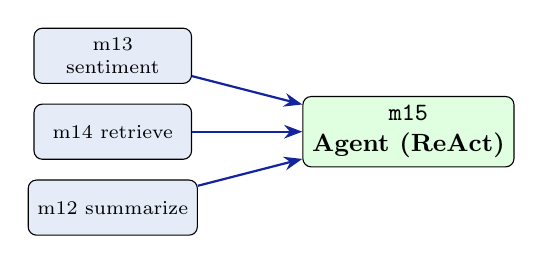
\begin{tikzpicture}[
      mod/.style={draw, fill=cnubluebg, rounded corners=3pt,
                  minimum width=2.0cm, minimum height=0.7cm,
                  font=\scriptsize, align=center},
      fin/.style={draw, fill=green!12, rounded corners=3pt,
                  minimum width=2.3cm, minimum height=0.7cm,
                  font=\small\bfseries, align=center},
      arr/.style={-{Stealth}, thick, color=cnublue}
  ]
    \node[mod] (t1) {m13\\ sentiment};
    \node[mod, below=0.25cm of t1] (t2) {m14 retrieve};
    \node[mod, below=0.25cm of t2] (t3) {m12 summarize};
    \node[fin, right=1.4cm of t2] (m15) {\texttt{m15}\\ Agent (ReAct)};
    \draw[arr] (t1)--(m15); \draw[arr] (t2)--(m15); \draw[arr] (t3)--(m15);
  \end{tikzpicture}
  \end{center}
  \vspace{3pt}
  \begin{columns}[T]
    \begin{column}{0.50\textwidth}
      \textbf{P15 da qurasiz:}\\[3pt]
      \small
      \begin{itemize}\setlength\itemsep{2pt}
        \item \texttt{m15 DocumentAssistantAgent}: ReAct $+$ 5 tool
        \item m13/m14/m12/m04/m10 ni \texttt{Tool} qilib ulash
        \item o'zbekcha so'rovga yakuniy javob
      \end{itemize}
    \end{column}
    \begin{column}{0.46\textwidth}
      \textbf{Birinchi assert (bu slayd [I1]):}\\[4pt]
      \small\ttfamily
      assert tool ==\\
      \phantom{xx}"sentiment\_classify"\\
      assert conf > 0.7\\[4pt]
      \normalfont\footnotesize\color{halfgray}
      \textit{\# Ma'ruza L15 [I1]-slayd bilan}\\
      \textit{\# solishtiring (ReAct tool tanlash)}
    \end{column}
  \end{columns}
\end{frame}

% ----------------------------------------------------------------
% [R] ADABIYOTLAR
% ----------------------------------------------------------------
\begin{frame}{Adabiyotlar}
  \begin{enumerate}\small\setlength\itemsep{5pt}
    \item Yao, S., va boshq.\ (2022). \textit{ReAct: Synergizing Reasoning and
          Acting in Language Models.} ICLR 2023.
    \item Schick, T., va boshq.\ (2023). \textit{Toolformer: Language Models Can
          Teach Themselves to Use Tools.} NeurIPS 2023.
    \item Wei, J., va boshq.\ (2022). \textit{Chain-of-Thought Prompting Elicits
          Reasoning in LLMs.} NeurIPS 2022.
    \item \texttt{python.langchain.com} --- Agents va Tools hujjatlari.
    \item \texttt{fastapi.tiangolo.com} --- API joylashtirish hujjatlari.
  \end{enumerate}
\end{frame}

% ================================================================
% [S] ILOVALAR (appendix --- slayd soniga kirmaydi)
% ================================================================
\appendix

\begin{frame}[fragile]{Ilova S1: ReAct prompt shabloni (qisqacha)}
  \small
  ReAct LLM ga quyidagi formatda fikrlashni so'raydi:
\begin{lstlisting}
Savol: {query}
Thought: men nima qilishim kerak?
Action: {tool_name}
Action Input: {args}
Observation: {tool natijasi}
... (takrorlanadi) ...
Thought: endi javobni bilaman
Final Answer: {yakuniy javob}
\end{lstlisting}
  \bunda{Model shu formatga amal qiladi; tizim Action/Action Input ni o'qib
  vositani chaqiradi, natijani Observation ga qo'yadi.}
\end{frame}

\begin{frame}{Ilova S2: agent xotirasi (memory)}
  \small
  Ko'p qadamli yoki ko'p navbatli (multi-turn) suhbatda agent \textbf{xotira}
  saqlaydi:
  \begin{itemize}\setlength\itemsep{2pt}
    \item \textbf{Qisqa muddatli}: joriy ReAct tarixi ($h_t$).
    \item \textbf{Uzoq muddatli}: oldingi suhbatlar (ko'pincha vektor DB da, L14).
  \end{itemize}
  \bunda{Xotira agentga oldingi qadamlar va suhbatlarni eslab, izchil javob
  berishga yordam beradi --- ammo kontekst oynasi va narxni oshiradi (L14 [I2]).}
\end{frame}

\end{document}
